\caulc
\begin{ex}%[TDMZZ26]%[Nguyễn Tấn Linh]%[1D2N3-4]
	Cho cấp số nhân $(u_{n})$ có $u_{1}=1$ và công bội $q=2$. Giá trị của $u_{4}$ bằng
	\choice
	{\True $8$}
	{$7$}
	{$16$}
	{$9$}
	\loigiai{
		Ta có $u_4=u_1\cdot q^3 = 1\cdot 2^3=8$.
	}
\end{ex}

\begin{ex}%[TDMZZ26]%[Nguyễn Tấn Linh]%[1D6N3-2]
	Tập xác định của hàm số $y=(2-x)^{\pi}$ là
	\choice
	{\True $(-\infty;2)$}
	{$(-\infty;+\infty)$}
	{$(0;+\infty)$}
	{$(2;+\infty)$}
	\loigiai{
		Hàm số $y=(2-x)^{\pi}$ có số mũ $\pi$ không nguyên nên điều kiện xác định là
		\[2-x>0 \Leftrightarrow x<2.\]
		Vậy tập xác định của hàm số là $\mathscr{D}=(-\infty;2)$.
	}
\end{ex}

\begin{ex}%[TDMZZ26]%[Nguyễn Tấn Linh]%[1H8H5-4]
	Cho hình lập phương $ABCD. A'B'C'D'$ có cạnh bằng $a$. Hãy tính $\mathrm{d}(AB,C'D')$.
	\begin{center}
		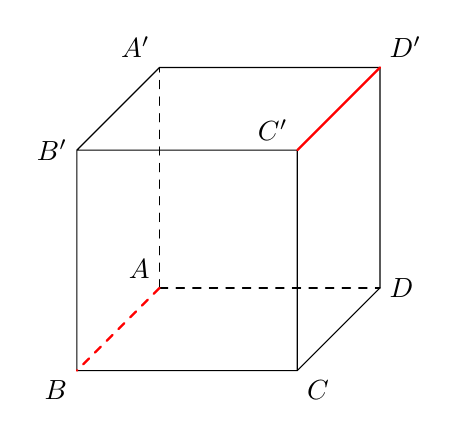
\begin{tikzpicture}[line join=round, line cap=round, scale=0.7]
			\coordinate (A)  at (1.5, 1.5);
			\coordinate (B)  at (0, 0);
			\coordinate (C)  at (4, 0);
			\coordinate (D)  at (5.5, 1.5);
			\coordinate (A') at (1.5, 5.5);
			\coordinate (B') at (0, 4);
			\coordinate (C') at (4, 4);
			\coordinate (D') at (5.5, 5.5);
			\draw[dashed] (A) -- (D)	 (A) -- (A');
			\draw (B) -- (C) -- (D) -- (D') -- (A') -- (B') -- cycle
			(B) -- (B') (C) -- (C') (A') -- (D') (C') -- (B');
			\draw[dashed, thick, red] (A) -- (B);
			\draw[thick, red] (C') -- (D');
			\node[above left] at (A) {$A$};
			\node[below left] at (B) {$B$};
			\node[below right] at (C) {$C$};
			\node[right] at (D) {$D$};
			\node[above left] at (A') {$A'$};
			\node[left] at (B') {$B'$};
			\node[above left] at (C') {$C'$};
			\node[above right] at (D') {$D'$};
		\end{tikzpicture}
	\end{center}
	\choice
	{$a$}
	{$a\sqrt{3}$}
	{\True $a\sqrt{2}$}
	{$\dfrac{a\sqrt{2}}{2}$}
	\loigiai{
		Ta có $AB \parallel CD$ và $CD \parallel C'D'$ nên $AB \parallel C'D'$.\\
		Do đó $\mathrm{d}(AB,C'D') = \mathrm{d}(B,C'D') = BC'$ (vì $C'D' \perp (BCC'B') \Rightarrow C'D' \perp BC'$).\\
		Vì $BCC'B'$ là hình vuông cạnh $a$ nên $BC'=a\sqrt{2}$.\\
		Vậy $\mathrm{d}(AB,C'D')=a\sqrt{2}$.
	}
\end{ex}

\begin{ex}%[TDMZZ26]%[Nguyễn Tấn Linh]%[1D7N1-2]
	Cho hàm số $f(x)=x^{2}-2x+3$. Số gia của hàm số $f(x)$ tại điểm $x_{0}=2$ ứng với số gia của biến số $\Delta x=0{,}1$ bằng
	\choice
	{$-1{,}8$}
	{$0{,}01$}
	{$2{,}1$}
	{\True $0{,}21$}
	\loigiai{
		Ta có $\Delta y = f(x_0+\Delta x) - f(x_0) = f(2+0{,}1) - f(2) = f(2{,}1) - f(2)$.\\
		Với $f(2{,}1) = (2{,}1)^2 - 2\cdot 2{,}1 + 3 = 3{,}21$.\\
		Với $f(2) = 2^2 - 2\cdot 2 + 3 = 3$.\\
		Vậy $\Delta y = 3{,}21 - 3 = 0{,}21$.
	}
\end{ex}

\begin{ex}%[TDMZZ26]%[Nguyễn Tấn Linh]%[1H8N7-6]
	Cho hình chóp cụt đều $ABCD. A'B'C'D'$ có hai cạnh đáy bằng $4$ và $6$, khoảng cách hai đáy bằng $3$. Hãy tính thể tích của hình chóp cụt đều $ABCD. A'B'C'D'$.
	\choice
	{$228$}
	{$38$}
	{\True $76$}
	{$114$}
	\loigiai{
		Diện tích hai đáy của hình chóp cụt đều lần lượt là $S_1 = 4^2 = 16$ và $S_2 = 6^2 = 36$.\\
		Chiều cao của hình chóp cụt là $h=3$.\\
		Thể tích của hình chóp cụt đều là
		\[ V = \dfrac{1}{3}h\left(S_1 + S_2 + \sqrt{S_1S_2}\right) = \dfrac{1}{3}\cdot 3\cdot \left(16+36+\sqrt{16\cdot 36}\right) = 76. \]
	}
\end{ex}

\begin{ex}%[TDMZZ26]%[Nguyễn Tấn Linh]%[2D1N2-2]
	Cho bảng biến thiên của hàm số $f(x)$ như hình vẽ bên dưới.
	\begin{center}
		
\begin{tikzpicture}[>=stealth]
			\tkzTabInit[nocadre=false,lgt=1.2,espcl=3,deltacl=0.5]{$x$/.7,$f'(x)$/.7,$f(x)$/2}
			{$-\infty$, $-2$, $0$, $+\infty$}
			\tkzTabLine{ , +, $0$, -, $0$, +, }
			\tkzTabVar{-/$-\infty$, +/$3$, -/$1$, +/$+\infty$}
		\end{tikzpicture}
	\end{center}
	Điểm cực tiểu của đồ thị hàm số $y=f(x)$ là
	\choice
	{\True $(0;1)$}
	{$x=0$}
	{$y=1$}
	{$(-2;3)$}
	\loigiai{
		Dựa vào bảng biến thiên, đồ thị hàm số đạt cực tiểu tại $x=0$ và giá trị cực tiểu là $y=1$.\\
		Vậy điểm cực tiểu của đồ thị hàm số là $(0;1)$.
	}
\end{ex}

\begin{ex}%[TDMZZ26]%[Nguyễn Tấn Linh]%[1D5N1-3]
	Cho mẫu số liệu ghép nhóm $M$ với bảng tần số ghép nhóm như sau:
	\begin{center}
		\begin{tabular}{|l|c|c|c|c|c|c|}
			\hline
			Nhóm & $[8;10)$ & $[10;12)$ & $[12;14)$ & $[14;16)$ & $[16;18)$ & $[18;20)$ \\
			\hline
			Tần số & $6$ & $2$ & $8$ & $4$ & $6$ & $4$ \\
			\hline
		\end{tabular}
	\end{center}
	Hãy xác định số trung bình cộng của mẫu số liệu ghép nhóm $M$ (làm tròn kết quả đến hàng phần mười).
	\choice
	{$\overline{x}=15{,}1$}
	{\True $\overline{x}=13{,}9$}
	{$\overline{x}=15$}
	{$\overline{x}=12{,}8$}
	\loigiai{
		Ta có bảng giá trị đại diện của mẫu số liệu:
		\begin{center}
			\begin{tabular}{|l|c|c|c|c|c|c|}
				\hline
				Nhóm & $[8;10)$ & $[10;12)$ & $[12;14)$ & $[14;16)$ & $[16;18)$ & $[18;20)$ \\
				\hline
				Giá trị đại diện $x_i$ & $9$ & $11$ & $13$ & $15$ & $17$ & $19$ \\
				\hline
				Tần số $f_i$ & $6$ & $2$ & $8$ & $4$ & $6$ & $4$ \\
				\hline
			\end{tabular}
		\end{center}
		Cỡ mẫu $N = 6+2+8+4+6+4=30$.\\
		Số trung bình cộng của mẫu số liệu là
		\[ \overline{x} = \dfrac{9\cdot 6 + 11\cdot 2 + 13\cdot 8 + 15\cdot 4 + 17\cdot 6 + 19\cdot 4}{30} = \dfrac{418}{30} \approx 13{,}9. \]
	}
\end{ex}

\begin{ex}%[TDMZZ26]%[Nguyễn Tấn Linh]%[2D4N1-1]
	Nếu $f(x)=x^{3}-2x^{2}+2026$ là một nguyên hàm của hàm số $F(x)$ thì biểu thức $F'(x)$ tương ứng là
	\choice
	{$F'(x)=x^{3}-2x^{2}+2026$}
	{$F'(x)=3x^{2}-4x$}
	{\True $F'(x)=6x-4$}
	{$F'(x)=\dfrac{x^{4}}{4}-\dfrac{2x^{3}}{3}+2026x$}
	\loigiai{
		Vì $f(x)$ là một nguyên hàm của hàm số $F(x)$ nên ta có
		\[ F(x) = f'(x) = 3x^2-4x. \]
		Đạo hàm của hàm số $F(x)$ là
		\[ F'(x) = (3x^2-4x)' = 6x-4. \]
	}
\end{ex}

\begin{ex}%[TDMZZ26]%[Nguyễn Tấn Linh]%[2H5N1-2]
	Trong không gian $Oxyz$, một vectơ pháp tuyến của mặt phẳng $(P)\colon 2x-z+2=0$ tương ứng là
	\choice
	{$\overrightarrow{n}_{1}=(2;-1;2)$}
	{\True $\overrightarrow{n}_{2}=(2;0;-1)$}
	{$\overrightarrow{n}_{3}=(2;0;0)$}
	{$\overrightarrow{n}_{4}=(2;0;2)$}
	\loigiai{
		Mặt phẳng $(P)\colon 2x-z+2=0$ có một vectơ pháp tuyến là $\overrightarrow{n}_{2}=(2;0;-1)$.
	}
\end{ex}

\begin{ex}%[TDMZZ26]%[Nguyễn Tấn Linh]%[2H2N1-2]
	Cho hình lăng trụ đứng $ABC. A'B'C'$. Hỏi khi đó $\overrightarrow{AB}+\overrightarrow{AA'}+\overrightarrow{BC}$ bằng với véc-tơ nào dưới đây?
	\begin{center}
		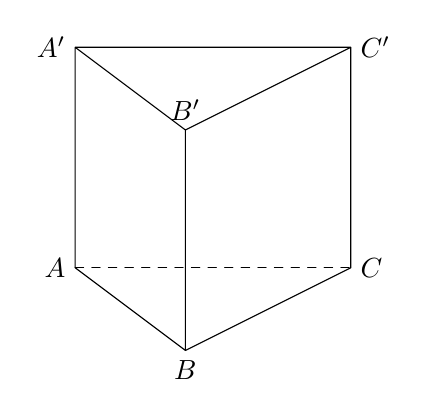
\begin{tikzpicture}[line join=round, line cap=round, scale=0.7]
			\coordinate (A) at (0,0);
			\coordinate (B) at (2,-1.5);
			\coordinate (C) at (5,0);
			\coordinate (A') at (0,4);
			\coordinate (B') at (2,2.5);
			\coordinate (C') at (5,4);
			\draw[dashed] (A) -- (C);
			\draw (A) -- (B) -- (C)  (A') -- (B') -- (C') -- cycle  (A) -- (A')  (B) -- (B')  (C) -- (C');
			\node[left] at (A) {$A$};
			\node[below] at (B) {$B$};
			\node[right] at (C) {$C$};
			\node[left] at (A') {$A'$};
			\node[above] at (B') {$B'$};
			\node[right] at (C') {$C'$};
		\end{tikzpicture}
	\end{center}
	\choice
	{$\overrightarrow{AB'}$}
	{$\overrightarrow{CC'}$}
	{\True $\overrightarrow{AC'}$}
	{$\overrightarrow{0}$}
	\loigiai{
		Ta có $\overrightarrow{AB}+\overrightarrow{AA'}+\overrightarrow{BC} = \left(\overrightarrow{AB}+\overrightarrow{BC}\right) + \overrightarrow{AA'} = \overrightarrow{AC} + \overrightarrow{CC'} = \overrightarrow{AC'}$.
	}
\end{ex}

\begin{ex}%[TDMZZ26]%[Nguyễn Tấn Linh]%[2D1H4-1]
	Số đường tiệm cận (tính cả tiệm cận đứng, tiệm cận ngang, tiệm cận xiên) của đồ thị hàm số $y=\sqrt{x^{2}+2x}+\dfrac{x^{2}+1}{x}$ là
	\choice
	{$2$}
	{$1$}
	{$0$}
	{\True $3$}
	\loigiai{
		Tập xác định của hàm số là $\mathscr{D}=(-\infty;-2]\cup (0;+\infty)$.\\
		Tiệm cận đứng:
		\[ \lim\limits_{x\to 0^+} y = \lim\limits_{x\to 0^+} \left(\sqrt{x^2+2x}+\dfrac{x^2+1}{x}\right) = +\infty. \]
		Suy ra đường thẳng $x=0$ là tiệm cận đứng của đồ thị hàm số.\\
		Tiệm cận ngang và tiệm cận xiên:
		\begin{itemize}
			\item Khi $x \to +\infty$: Ta có $y = \sqrt{x^2+2x} + x + \dfrac{1}{x}$.\\
			$\lim\limits_{x\to +\infty} \dfrac{y}{x} = \lim\limits_{x\to +\infty} \left(\sqrt{1+\dfrac{2}{x}} + 1 + \dfrac{1}{x^2}\right) = 2$.\\
			$\lim\limits_{x\to +\infty} (y-2x) = \lim\limits_{x\to +\infty} \left(\sqrt{x^2+2x} - x + \dfrac{1}{x}\right) = \lim\limits_{x\to +\infty} \left(\dfrac{2x}{\sqrt{x^2+2x}+x} + \dfrac{1}{x}\right) = 1$.\\
			Suy ra đường thẳng $y=2x+1$ là tiệm cận xiên của đồ thị hàm số khi $x \to +\infty$.
			\item Khi $x \to -\infty$: Ta có
			\begin{eqnarray*}
				\lim\limits_{x\to -\infty} y &=& \lim\limits_{x\to -\infty} \left(\sqrt{x^2+2x} + x + \dfrac{1}{x}\right) = \lim\limits_{x\to -\infty} \left(\dfrac{x^2+2x-x^2}{\sqrt{x^2+2x}-x} + \dfrac{1}{x}\right)\\
				&=& \lim\limits_{x\to -\infty} \left(\dfrac{2x}{-x\sqrt{1+\dfrac{2}{x}}-x} + \dfrac{1}{x}\right) = \lim\limits_{x\to -\infty} \left(\dfrac{2}{-\sqrt{1+\dfrac{2}{x}}-1} + \dfrac{1}{x}\right) = -1.
			\end{eqnarray*}
			Suy ra đường thẳng $y=-1$ là tiệm cận ngang của đồ thị hàm số khi $x \to -\infty$.
		\end{itemize}
		Vậy đồ thị hàm số có tổng cộng $3$ đường tiệm cận.
	}
\end{ex}
\cauds
\begin{ex}%[TDMZZ26]%[Nguyễn Tấn Linh]%[2D4H2-1]
	Cho biết giá trị $\displaystyle\int\limits_{0}^{1}\left[2f(x)+3g(x)\right]\mathrm{\,d}x=5$ và $\displaystyle\int\limits_{0}^{1}\left[5f(x)-3g(x)\right]\mathrm{\,d}x=2$. Hãy đi tính giá trị của tích phân $I=\displaystyle\int\limits_{0}^{1}\left[f(x)-2x\right]\mathrm{\,d}x$.
	\choice
	{\True $0$}
	{$-2$}
	{$4$}
	{$3$}
	\loigiai{
		Từ giả thiết, ta có hệ phương trình
		\[ \heva{&2\displaystyle\int\limits_{0}^{1}f(x)\mathrm{\,d}x + 3\displaystyle\int\limits_{0}^{1}g(x)\mathrm{\,d}x = 5\\ &5\displaystyle\int\limits_{0}^{1}f(x)\mathrm{\,d}x - 3\displaystyle\int\limits_{0}^{1}g(x)\mathrm{\,d}x = 2} \Rightarrow 7\displaystyle\int\limits_{0}^{1}f(x)\mathrm{\,d}x = 7 \Leftrightarrow \displaystyle\int\limits_{0}^{1}f(x)\mathrm{\,d}x = 1. \]
		Khi đó, tích phân cần tính là
		\[ I = \displaystyle\int\limits_{0}^{1}f(x)\mathrm{\,d}x - \displaystyle\int\limits_{0}^{1}2x\mathrm{\,d}x = 1 - x^2\bigg|_0^1 = 1 - 1 = 0. \]
	}
\end{ex}

\begin{ex}%[2D1H5-7]%[Dương Công Tạo]
	Trong mặt phẳng toạ độ Oxy, cho hàm số $y = f (x) = x^{11} -11x$ có đồ thị $(C)$.
	\choiceTF
	{\True $f'(x)=11x^{10} -11$}
	{\True $f(x)$ nghịch biến trên nửa khoảng $[-1;1)$}
	{\True $(C)$ có tâm đối xứng là $(0;0)$}
	{\True $(C)$ có hai điểm cực trị cách nhau một khoảng bằng $2\sqrt{101}$}
	\loigiai{
		Xét hàm số $y = f (x) = x^{11} -11x$ trên khoảng $(-\infty;+\infty)$.
		\begin{itemchoice}
			\itemch Ta có $f'(x) = 11x^{10} -11$.
			\itemch Ta có $f'(x) = 11x^{10} -11$; $f'(x)=0\Leftrightarrow 11x^{10} -11=0\Leftrightarrow x=\pm 1$.\\
			Bảng biến thiên
			\begin{center}
				
\begin{tikzpicture}[>=stealth]
					\tkzTabInit[nocadre=false,lgt=1.5,espcl=2,deltacl=0.6]{$x$/.7 ,$f'(x)$/.7,$f(x)$/2}
					{$-\infty$ , $-1$ , $1$ , $+\infty$}
					\tkzTabLine{ , + , $0$ , - , $0$ , + , }
					\tkzTabVar{-/$-\infty$ , +/$10$ , -/$-10$ , +/$+\infty$}
				\end{tikzpicture}
			\end{center}
			Vì $f(x)$ là hàm đa thức nên nó xác định là liên tục trên khoảng $(-\infty;+\infty)$ nên nó liên tục tại $x=-1$. Kết hợp với bảng biến thiên suy ra $f(x)$ nghịch biến trên nửa khoảng $[-1;1)$.
			\itemch Vì $f(x)$ là hàm số lẻ nên đồ thị $(C)$ nhận gốc toạ độ $O$ làm tâm đối xứng.
			\itemch Gọi $A(-1;10)$ và $B(1;-10)$ là hai điểm cực trị của đồ thị $(C)$.\\
			Ta có $AB=\sqrt{(1+1)^2+(-10-10)^2=2\sqrt{101}}$.
		\end{itemchoice}
	}
\end{ex}

\begin{ex}%[TDMZZ26]%[Hà Văn Hảo]%[2D6H1-2]
	Gọi $A$ và $B$ là hai biến cố của một phép thử có không gian mẫu là $\Omega$. Biết rằng $\mathrm{P}(A) = 0{,}6$; $\mathrm{P}(\overline{A}B) = 0{,}36$; $\mathrm{P}(A\overline{B}) = 0{,}48$.
	\choiceTF
	{\True $\mathrm{P}(\overline{A}) = 0{,}4$}
	{\True $\mathrm{P}(B \mid \overline{A}) = 0{,}9$}
	{\True $\mathrm{P}(B) = 0{,}48$}
	{$\mathrm{P}(B \mid A) = 0{,}25$}
	\loigiai{
		\begin{itemchoice}
			\itemch Ta có $\mathrm{P}(\overline{A}) = 1 - \mathrm{P}(A) = 1 - 0{,}6 = 0{,}4$.
			\itemch Ta có $\mathrm{P}(B \mid \overline{A}) = \dfrac{\mathrm{P}(\overline{A}B)}{\mathrm{P}(\overline{A})} = \dfrac{0{,}36}{0{,}4} = 0{,}9$.
			\itemch Trước hết, ta tính $\mathrm{P}(AB)$.\\
			Vì $A = (AB) \cup (A\overline{B})$ và hai biến cố này xung khắc, nên
			\[\mathrm{P}(A) = \mathrm{P}(AB) + \mathrm{P}(A\overline{B}) \Rightarrow \mathrm{P}(AB) = \mathrm{P}(A) - \mathrm{P}(A\overline{B}) = 0{,}6 - 0{,}48 = 0{,}12.\]
			Khi đó $\mathrm{P}(B) = \mathrm{P}(AB) + \mathrm{P}(\overline{A}B) = 0{,}12 + 0{,}36 = 0{,}48$.
			\itemch Ta có $\mathrm{P}(B \mid A) = \dfrac{\mathrm{P}(AB)}{\mathrm{P}(A)} = \dfrac{0{,}12}{0{,}6} = 0{,}2 \neq 0{,}25$.
		\end{itemchoice}
	}
\end{ex}

\begin{ex}%[2D4V3-5]%[TDMZZ26]%[Vũ Hồng Toàn]
	Cho một bể chứa nước và ban đầu chưa có nước. Người ta bắt đầu bơm nước vào bể với lưu lượng là $L_1(t) = 4t + 3$\,(lít/phút). Cùng lúc đó, do bể có một vết nứt dưới đáy nên nước bị chảy ra ngoài với lưu lượng là $L_2(t) = t$\,(lít/phút). Quá trình được xét trong $28$\,phút đầu tiên (tính từ thời điểm $t = 0$ đến $t = 28$\,phút). Dung tích tối đa của bể là $950$\,lít.
	\choiceTF
	{\True Thể tích nước được bơm vào bể trong $10$ phút đầu tiên là $230$\,(lít)}
	{Tại thời điểm $t = 15$\,phút nước trong bể là $495$\,lít}
	{\True Khi nước chảy vào vừa làm đầy bể, thì đã có $292$\,lít nước bị chảy ra ngoài (làm tròn kết quả đến hàng đơn vị)}
	{Tính trong khoảng thời gian $28$\,phút đầu tiên, trung bình cứ $1$\,phút sẽ có $25$\,lít nước bị chảy ra ngoài (làm tròn kết quả đến hàng phần đơn vị)}
	\loigiai{
		\begin{itemchoice}
			\itemch Thể tích nước được bơm vào bể trong $10$\,phút đầu tiên là
			\[V_{\text{in}}(10) = \displaystyle\displaystyle\int\limits_{0}^{10} L_1(t) \mathrm{\,d}t = \displaystyle\int\limits_{0}^{10} \left(4t + 3\right) \mathrm{\,d}t = \left(2t^2 + 3t\right)\bigg|_{0}^{10} = 230 \text{ (lít)}.\]
			\itemch Lưu lượng nước trong bể tại thời điểm $t$ là
			\[L(t) = L_1(t) - L_2(t) = (4t + 3) - t = 3t + 3 \text{ (lít/phút).}\]
			Thể tích nước trong bể tại thời điểm $t = 15$\,phút là
			\[V(15) = \displaystyle\int\limits_{0}^{15} \left(3t + 3\right) \mathrm{\,d}t = \left( \dfrac{3t^2}{2} + 3t \right) \Bigg|_{0}^{15} = 382{,}5 \text{ (lít)}.\]
			\itemch Thời điểm nước vừa làm đầy bể ($V(t) = 950$\,lít) thỏa mãn phương trình
			\allowdisplaybreaks
			\begin{eqnarray*}
				&&\displaystyle\int\limits_{0}^{t} (3x + 3) \mathrm{\,d}x = 950 \\
				&\Leftrightarrow& \dfrac{3t^2}{2} + 3t = 950 \\
				&\Leftrightarrow& 3t^2 + 6t - 1900 = 0 \\
				&\Leftrightarrow& \hoac{&t \approx 24{,}186&\text{ (nhận)}\\&t \approx -26{,}186&\text{ (loại)}.}
			\end{eqnarray*}
			Thể tích nước bị chảy ra ngoài cho đến khi bể đầy là
			\[V_{\text{out}} = \displaystyle\int\limits_{0}^{24{,}186} x \mathrm{\,d}x = \dfrac{x^2}{2} \Bigg|_{0}^{24{,}186} \approx 292 \text{ (lít)}.\]
			\itemch Lượng nước chảy ra ngoài trong $28$\,phút đầu tiên là
			\[V_{\text{out}}(28) = \displaystyle\int\limits_{0}^{28} t \mathrm{\,d}t = \dfrac{t^2}{2} \Bigg|_{0}^{28} = 392 \text{ (lít)}.\]
			Trung bình mỗi phút lượng nước chảy ra ngoài là
			\[\overline{V}_{\text{out}} = \dfrac{392}{28} = 14 \text{ (lít/phút).}\]
		\end{itemchoice}
	}
\end{ex}

\begin{ex}%[2H5V3-4]%[TDMZZ26]%[Văn Minh Thoại]
	Trong không gian $Oxyz$ có đơn vị dài trên mỗi trục là kilômét và mặt đất là mặt phẳng tọa độ $(Oxy)$, có một trạm thu phát sóng điện thoại di động được đặt ở vị trí $I(-4;6;0{,}2)$ được thiết kế với bán kính phủ sóng là $5$ km.
	\choiceTF
	{\True Phương trình mặt cầu $(S)$ mô tả ranh giới bên ngoài của vùng phủ sóng trong không gian là $(x+4)^2+(y-6)^2+(z-0{,}2)^2=25$}
	{\True Khoảng cách xa nhất giữa hai điểm thuộc vùng phủ sóng là $10$ km}
	{\True Người dùng điện thoại ở vị trí $A$ có tọa độ là $(-4;0;0)$ không thể sử dụng dịch vụ của trạm thu phát sóng đã cho}
	{Trong điều kiện giao thông thuận lợi, khoảng cách ngắn nhất để một người ở vị trí $A$ di chuyển tới vùng phủ sóng là $1\,003$ m \textit{(tính theo đơn vị mét và làm tròn kết quả đến hàng đơn vị)}}
	\loigiai{
		\begin{itemchoice}
			\itemch Phương trình ranh giới bên ngoài của vùng phủ sóng là mặt cầu tâm $I(-4;6;0{,}2)$ và bán kính $R=5$ có phương trình dạng
			\[(x+4)^2+(y-6)^2+(z-0{,}2)^2=25.\]
			\itemch Khoảng cách xa nhất giữa hai điểm thuộc vùng phủ sóng trong không gian chính là độ dài đường kính của mặt cầu $(S)$.\\
			Do đó khoảng cách lớn nhất là $2R=10$ km.
			\itemch Khoảng cách từ vị trí $A(-4;0;0)$ đến tâm phát sóng $I$ là
			\[IA=\sqrt{(-4+4)^2+(6-0)^2+(0{,}2-0)^2}=\sqrt{36+0{,}04}=\sqrt{36{,}04}\approx 6{,}0033\mathrm{\,km}.\]
			Do $IA>R$ nên điểm $A$ nằm ngoài khối cầu $(S)$, người dùng tại $A$ không nằm trong vùng phủ sóng nên không thể sử dụng dịch vụ.
			\itemch
			\begin{center}
				\begin{tikzpicture}[declare function={R=3.9; h=1.5; r=sqrt (R*R-h*h); ry=r*0.35; ang=225; kA=1.4;},line join=round,line cap=round,>=stealth,scale=1,font=\footnotesize]
					\draw (3,4)--(6,4)--(4,-3)--(-6,-3) -- (-4,4)--(-3,4);
					\draw[dashed] (-3,4)--(3,4);
					\node at (4.5,3) {$(Oxy)$};
					\path (0,0) coordinate (Ip);
					\path (0,h) coordinate (I);
					\path ({r*cos (ang)},{ry*sin (ang)}) coordinate (M);
					\path ({kA*r*cos (ang)},{kA*ry*sin (ang)}) coordinate (A);
					\begin{scope}
						\clip plot[domain=0:360,samples=150] ({r*cos (\x)},{ry*sin (\x)});
						\draw[pattern={Lines[angle=45,distance=3pt,line width=0.3pt]},pattern color=gray!70,draw=none] (-5,-5) rectangle (5,5);
					\end{scope}
					\draw[dashed] plot[domain=0:180,samples=150] ({r*cos (\x)},{ry*sin (\x)});
					\draw plot[domain=180:360,samples=150] ({r*cos (\x)},{ry*sin (\x)});
					\draw (I) circle (R);
					\draw ($(I)+(0:R)$) arc (0:-180:{R} and {0.2*R});
					\draw[dashed] ($(I)+(0:R)$) arc (0:180:{R} and {0.2*R});
					\draw[dashed] (I) -- (Ip) node[pos=0.35,sloped,above] {$0{,}2$};
					\draw[dashed] (Ip) -- (M) node[pos=0.6,sloped,below] {$r$};
					\draw[dashed] (I) -- (M) node[pos=0.5,sloped,below] {$R=5$}; \draw[dashed] (I) -- (A);
					
					\draw (M) -- (A) node[pos=0.5,sloped,below] {$d$};
					\path pic[draw,line width=0.6pt,angle radius=5pt]{right angle=I--Ip--M};
					\foreach \p/\pos/\t in {I/90/I,Ip/-15/I',M/-65/M,A/-90/A}{
						\draw[fill,ball color=red] (\p) circle (1pt) node[shift={(\pos:9pt)}] {$\t$};
					}
					\node[shift={(45:12pt)}] at ({R*cos (45)},{h+R*sin (45)}) {$(S)$};
					\node[shift={(-120:0.5)}] at ({r*cos (315)},{ry*sin (315)}) {$(C)$};
				\end{tikzpicture}
			\end{center}
			Vì người dùng di chuyển trong điều kiện giao thông thuận lợi trên mặt đất nên người đó chỉ di chuyển trên mặt phẳng tọa độ $(Oxy)$ có phương trình $z=0$.\\
			Giao tuyến của mặt cầu $(S)$ và mặt phẳng $(Oxy)$ là một đường tròn $(C)$ giới hạn vùng phủ sóng trên mặt đất.
			Thay $z=0$ vào phương trình mặt cầu ta được
			\[(x+4)^2+(y-6)^2+(0-0{,}2)^2=25 \Leftrightarrow (x+4)^2+(y-6)^2=24{,}96.\]
			Vùng phủ sóng trên mặt đất là hình tròn tâm $I'(-4;6;0)$ và bán kính $r=\dfrac{4\sqrt{39}}{5}$ km.
			\\
			Khoảng cách từ điểm $A(-4;0;0)$ đến $I'$ là
			\[AI'=\sqrt{(-4+4)^2+(6-0)^2+0^2}=6\mathrm{\,km}.\]
			Để tới vùng phủ sóng với khoảng cách ngắn nhất trên mặt đất, người đó cần di chuyển quãng đường $d$ từ $A$ hướng thẳng về phía tâm $I'$ cho đến khi chạm mép vùng phủ sóng (đường tròn $(C)$ tại điểm $M$). Khoảng cách ngắn nhất trên mặt đất là
			\[d=AI'-r=6-\dfrac{4\sqrt{39}}{5}=\dfrac{30-4\sqrt{39}}{5}\approx 1{,}004\mathrm{\,km}=1\,004\mathrm{\,m}.\]
			Do đó, khoảng cách ngắn nhất cần tìm là $1\,004$ m.
		\end{itemchoice}
	}
\end{ex}
\caukq
\begin{ex}%[1H3V4-3]%[TDMZZ26]%[Lê Hồ Quang Minh]
	\immini[thm]{Cho một miếng tôn hình chữ nhật $ABCD$ với độ dài các cạnh $AB = 100\text{ cm}$, $BC = 60\text{ cm}$. Ta tiến hành gấp miếng tôn theo các cạnh $MC, MD$ sao cho đến khi hai cạnh $MA$, $MB$ trùng nhau thì ta gọi hai điểm $A$ và $B$ là điểm $S$. Hãy tính theo đơn vị đêximét khối thể tích của tứ diện gấp được $SMCD$ \textit{(không làm tròn các kết quả trung gian, chỉ làm tròn kết quả cuối cùng đến hàng phần mười)}?
		\par\shortans[oly]{27,6}}
	{\begin{tikzpicture}[scale=1, font=\footnotesize, line join=round, line cap=round, >=stealth]
			\def\w{5.0}
			\def\h{3.0}
			\coordinate (D) at (0,0);
			\coordinate (C) at (\w,0);
			\coordinate (B) at (\w,\h);
			\coordinate (A) at (0,\h);
			\coordinate (M) at ($(A)!0.5!(B)$);
			\draw[line width=1pt, red!80!black] (A)--(B)--(C)--(D)--cycle;
			\draw[line width=0.8pt, dashed, blue!80!black] (M)--(D);
			\draw[line width=0.8pt, dashed, blue!80!black] (M)--(C);
			\node[below] at ($(D)!0.5!(C)$) {$100$};
			\node[right] at ($(C)!0.5!(B)$) {$60$};
			\foreach \i/\g in {A/135, B/45, C/-45, D/-135, M/90}
			\fill[black] (\i) circle (1pt) +(\g:2.5mm) node {$\i$};
	\end{tikzpicture}}
	\loigiai{
		\immini{
			Đổi $60$ cm $=6$ dm và $100$ cm $=10$ dm.\\
			Để sau khi gấp, hai cạnh $MA$ và $MB$ trùng nhau tạo thành cạnh $SM$ của tứ diện $SMCD$ thì $SM = MA = MB = 5$.\\
			Vì $DA=CB = 6$ nên sau khi gấp ta được tứ diện $SMCD$ có $SC=SD = 6$.\\
			Dễ thấy $\triangle SCD$ và $\triangle MCD$ lần lượt cân tại $S$ và $M$.\\
			Gọi $I$ là trung điểm cạnh $CD$.\\
			Ta có $\heva{&DC \perp SI\\&DC \perp MI} \Rightarrow DC \perp (SMI)$.\\
			Mà $DC \subset (MCD)$ nên $(SMI)\perp (MCD)$.
		}{
			\begin{tikzpicture}[scale=0.65, font=\footnotesize, line join=round, line cap=round, >=stealth]
				\coordinate (D) at (0,0);
				\coordinate (C) at (10,0);
				\coordinate (I) at ($(D)!0.5!(C)$);
				\coordinate (M) at ($(I)+(-1.5,-3)$);
				\coordinate (H) at ($(M)!0.6!(I)$);
				\coordinate (S) at ($(H)+(0,7)$);
				\draw (S)--(D)--(M)--(C)--cycle (M)--(S);
				\draw[dashed] (C)--(D) (M)--(I) (I)--(S)--(H);
				\pic[draw,thin,angle radius=2mm] {right angle = S--I--D} pic[draw,thin,angle radius=2mm] {right angle = M--I--D} pic[draw,thin,angle radius=2mm] {right angle = S--H--M};
				\foreach \i/\g in {D/-135, C/-45, M/-90, S/90,I/60,H/-30}
				\fill[black] (\i) circle (1pt) +(\g:2.5mm) node {$\i$};
			\end{tikzpicture}
		}
		\noindent Lại có $(SMI) \cap (MCD) = MI$ nên ta kẻ $SH \perp MI$, $H \in MI$.\\
		Suy ra $SH \perp (MCD)$.\\
		Ta lần lượt tính độ dài các cạnh như sau
		\begin{itemize}
			\item $MI = 6$ $\Rightarrow S_{MCD}=\dfrac{1}{2}\cdot MI \cdot DC = \dfrac{1}{2}\cdot 6 \cdot 10 = 30$.
			\item $SI=\sqrt{SD^2 - ID^2}=\sqrt{6^2 - 5^2}=\sqrt{11}$.
		\end{itemize}
		Nửa chu vi tam giác $SMI$ là $p=\dfrac{SI+MI+SM}{2}=\dfrac{\sqrt{11}+11}{2}$.\\
		Suy ra diện tích tam giác $SMI$ là $S_{SMI} = \sqrt{p\cdot(p-SM)\cdot(p-SI)\cdot(p-MI)}=\dfrac{5\sqrt{11}}{2}$.\\
		Khi đó $SH = \dfrac{2\cdot S_{SMI}}{MI} = \dfrac{5\sqrt{11}}{6}$.\\
		Vậy thể tích khối tứ diện $SMCD$ là
		\[V=\dfrac{1}{3}\cdot SH \cdot S_{MCD} = \dfrac{1}{3}\cdot \dfrac{5\sqrt{11}}{6}\cdot 30 = \dfrac{25\sqrt{11}}{3} \approx 27{,6}.\]
	}
\end{ex}

\begin{ex}%[1D6V3-5]%[TDMZZ25-19-TLN]%[Đỗ Đường Hiếu]
	Bác Hải mua một chiếc ti vi tại một cửa hàng với giá $30$ triệu đồng và đã trả trước $9$ triệu đồng ngay khi nhận ti vi. Số tiền còn lại bác lựa chọn trả góp trong vòng $12$ tháng với lãi suất $3\%$/tháng theo hình thức lãi kép trên dư nợ giảm dần, tiền lãi được tính dựa trên số dư nợ thực tế tại thời điểm tính lãi. Biết vào cuối mỗi tháng, bác Hải phải trả cho cửa hàng một số tiền không đổi là $m$ triệu đồng để sau đúng $12$ tháng thì hết nợ. Giá trị của $m$ bằng bao nhiêu triệu đồng (\textit{không làm tròn các kết quả trung gian, chỉ làm tròn kết quả cuối cùng đến hàng phần trăm})?
	\par\shortans{2,121}
	\loigiai{
		Số tiền bác Hải còn nợ sau khi trả trước là: $T = 30 - 9 = 21$ (triệu đồng).\\
		Gọi $r = 3\% = 0{,}03$ là lãi suất hàng tháng.\\
		Số tiền nợ còn lại sau mỗi tháng được tính theo công thức trả góp
		\begin{itemize}
			\item Sau tháng thứ nhất, số tiền nợ là $T_1 = T\cdot(1+r) - m$.
			\item Sau tháng thứ hai, số tiền nợ là
			$$T_2 = T_1(1+r) - m = T(1+r)^2 - m(1+r) - m.$$
			\item $\ldots\ldots\ldots$
			\item Sau tháng thứ $12$, số tiền nợ là
			\begin{eqnarray*}
				T_{12} &=& T(1+r)^{12} - m \left[ (1+r)^{11} + (1+r)^{10} + \dots + 1 \right]\\
				&=&T(1+r)^{12}-m \cdot \dfrac{1-(1+r)^{12}}{1-(1+r)}=T(1+r)^{12}-m \cdot \dfrac{(1+r)^{12}-1}{r}\\
				&=&21\cdot 1{,}03^{12}-m\cdot \dfrac{1{,}03^{12}-1}{0{,}03}.
			\end{eqnarray*}
		\end{itemize}
		Để sau $12$ tháng hết nợ thì
		$$T_{12} = 0\Leftrightarrow 21\cdot 1{,}03^{12}-m\cdot \dfrac{1{,}03^{12}-1}{0{,}03}=0\Leftrightarrow m = \dfrac{21 \cdot 0{,}03 \cdot 1{,}03^{12}}{1{,}03^{12} - 1} \approx 2{,}11.$$
		Vậy $m\approx 2{,}11$ (triệu đồng).
	}
\end{ex}

\begin{ex}%[0D0V2-9]%[TDMZZ26]%[Nguyễn Đức Tuấn Anh]
	\immini[thm]{
		Từ một bộ tú lơ khơ $52$ quân bài người ta bỏ đi $13$ chất bích và tất cả các con Át, rồi úp ngẫu nhiên mỗi quân vào một ô nhỏ hình chữ nhật được bố trí như hình vẽ. Gọi $p$ là xác suất để xếp được các ô tô màu có đúng $4$ chất rô và các ô được đánh chữ X có đúng $1$ chất rô. Hãy tính $10\,000p$ (\textit{làm tròn kết quả đến hàng đơn vị}).}{
		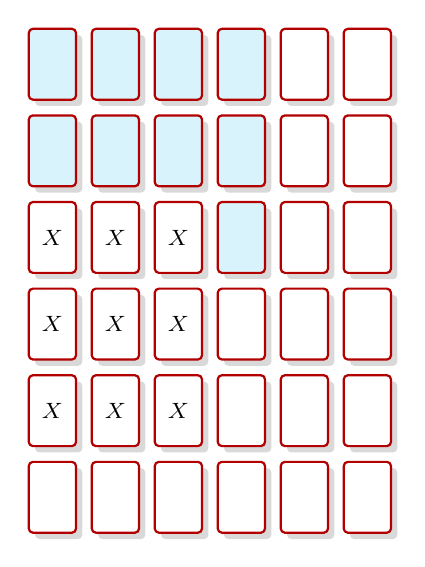
\begin{tikzpicture}[scale=1, font=\footnotesize, line join=round, line cap=round, >=stealth]
			\foreach \r in {1,...,6} {
				\foreach \c in {1,...,6} {
					\def\fillcol{white}
					\ifnum\r<3
					\ifnum\c<5 \def\fillcol{cyan!15} \fi
					\fi
					\ifnum\r=3
					\ifnum\c=4 \def\fillcol{cyan!15} \fi
					\fi
					\def\txt{}
					\ifnum\c<4
					\ifnum\r>2
					\ifnum\r<6 \def\txt{$X$} \fi
					\fi
					\fi
					\pgfmathsetmacro{\x}{\c*0.8}
					\pgfmathsetmacro{\y}{-\r*1.1}
					\def\w{0.3}
					\def\h{0.45}
					\fill[black!15, rounded corners=1.5pt] (\x-\w+0.08, \y-\h-0.08) rectangle (\x+\w+0.08, \y+\h-0.08);
					\draw[draw=red!70!black, thick, fill=\fillcol, rounded corners=1.5pt] (\x-\w, \y-\h) rectangle (\x+\w, \y+\h);
					\node at (\x, \y) {\txt};
				}
			}
		\end{tikzpicture}
	}
	\par\shortans{288}
	\loigiai{
		Bộ bài tú lơ khơ ban đầu có $52$ quân. Sau khi bỏ đi $13$ quân chất bích, bộ bài còn lại $39$ quân (gồm cơ, rô, nhép). Tiếp tục bỏ đi tất cả các con Át (gồm Át cơ, Át rô, Át nhép), số quân bài còn lại là $39 - 3 = 36$ quân.\\
		Trong $36$ quân bài này có $13 - 1 = 12$ quân chất rô và $24$ quân không phải chất rô.\\
		Quan sát lưới ô vuông trong hình vẽ (gồm $6$ hàng và $6$ cột, tổng cộng $36$ ô), ta nhận thấy
		\begin{itemize}
			\item Số ô được tô màu là $9$ ô (gồm $4$ ô ở hàng đầu tiên, $4$ ô ở hàng thứ hai và $1$ ô ở hàng thứ ba).
			\item Số ô được đánh chữ X là $9$ ô.
			\item Số ô còn lại (không tô màu và không có chữ X) là $36 - 9 - 9 = 18$ ô.
		\end{itemize}
		Việc úp ngẫu nhiên $36$ quân bài vào $36$ ô được xem như việc chọn ngẫu nhiên các ô để đặt quân bài. \\
		Số cách chọn $12$ ô từ $36$ ô để đặt $12$ quân bài chất rô là không gian mẫu $n(\Omega) = \mathrm{C}_{36}^{12}$.\\
		Gọi $A$ là biến cố \lq\lq Xếp được các ô tô màu có đúng $4$ chất rô và các ô được đánh chữ X có đúng $1$ chất rô\rq\rq.\\
		Để biến cố $A$ xảy ra, ta thực hiện các bước xếp $12$ quân rô như sau
		\begin{itemize}
			\item Chọn $4$ ô từ $9$ ô tô màu để đặt quân rô: có $\mathrm{C}_9^4$ cách.
			\item Chọn $1$ ô từ $9$ ô có chữ X để đặt quân rô: có $\mathrm{C}_9^1$ cách.
			\item Số quân rô còn lại là $12 - 4 - 1 = 7$ quân, ta chọn $7$ ô từ $18$ ô còn lại để đặt chúng: có $\mathrm{C}_{18}^7$ cách.
		\end{itemize}
		Số kết quả thuận lợi cho biến cố $A$ là $n(A) = \mathrm{C}_9^4 \cdot \mathrm{C}_9^1 \cdot \mathrm{C}_{18}^7$.\\
		Xác suất của biến cố $A$ là
		\[p = \dfrac{n(A)}{n(\Omega)} = \dfrac{\mathrm{C}_9^4 \cdot \mathrm{C}_9^1 \cdot \mathrm{C}_{18}^7}{\mathrm{C}_{36}^{12}} \approx 0{,}028832\]
		Suy ra $10\,000p \approx 288$.
	}
\end{ex}

\begin{ex}%[0D0C2-5]%[TDM42]
	Có hai rổ bi đựng những viên bi có cùng kích thước và cùng khối lượng. Rổ I có $4$ bi đỏ và $3$ bi xanh, rổ II có $5$ bi đỏ và $2$ bi xanh. Tiến hành đổ hết $7$ viên bi từ rổ I sang rổ II. Sau đó lại lấy ngẫu nhiên $7$ viên bi ở rổ II trở lại rổ I. Hãy tính xác suất để lấy được đúng ba viên bi từ rổ II về rổ I là của rổ I ban đầu, nếu biết đã lấy $4$ bi đỏ và $3$ bi xanh về rổ I \textit{(làm tròn kết quả đến hàng phần trăm)}?
	\begin{center}
		\begin{tikzpicture}[scale=0.8, >=stealth]
			% Rổ I
			\draw[thick, draw=black!100] (0,0) rectangle (3.5, 2.3);
			\node[font=\bfseries] at (1.75, 2.7) {Rổ I};
			\filldraw[fill=red, draw=yellow, thick] (0.7, 0.6) circle (0.25);
			\filldraw[fill=red, draw=yellow, thick] (1.3, 1.2) circle (0.25);
			\filldraw[fill=red, draw=yellow, thick] (2.2, 0.5) circle (0.25);
			\filldraw[fill=red, draw=yellow, thick] (3.0, 1.2) circle (0.25);
			\filldraw[fill=cyan, draw=yellow, thick] (1.5, 1.9) circle (0.25);
			\filldraw[fill=cyan, draw=yellow, thick] (2.3, 1.4) circle (0.25);
			\filldraw[fill=cyan, draw=yellow, thick] (3.0, 0.5) circle (0.25);
			
			% Rổ II
			\draw[thick, draw=black!100] (4.5,0) rectangle (8, 2.3);
			\node[font=\bfseries] at (6.25, 2.7) {Rổ II};
			\filldraw[fill=red, draw=yellow, thick] (5.1, 0.6) circle (0.25);
			\filldraw[fill=red, draw=yellow, thick] (5.2, 1.5) circle (0.25);
			\filldraw[fill=red, draw=yellow, thick] (6.0, 0.5) circle (0.25);
			\filldraw[fill=red, draw=yellow, thick] (6.8, 1.6) circle (0.25);
			\filldraw[fill=red, draw=yellow, thick] (7.4, 0.6) circle (0.25);
			\filldraw[fill=cyan, draw=yellow, thick] (6.0, 1.4) circle (0.25);
			\filldraw[fill=cyan, draw=yellow, thick] (6.6, 0.9) circle (0.25);
		\end{tikzpicture}
	\end{center}
	\par\shortans[0]{0,34}
	\loigiai{
		Gọi $A$ là biến cố: ``Lấy được $4$ bi đỏ và $3$ bi xanh từ rổ II về rổ I''.\\
		Gọi $B$ là biến cố: ``Lấy được đúng $3$ viên bi thuộc rổ I ban đầu''.\\
		Bài toán yêu cầu tính xác suất có điều kiện: $P(B|A) = \dfrac{n(A \cap B)}{n(A)}$.\\
		\textbf{Bước 1: Tính số phần tử của biến cố $A$}\\
		Sau khi đổ hết $7$ viên bi từ rổ I sang rổ II, rổ II có tổng cộng $14$ viên bi, gồm:
		\begin{itemize}
			\item Số bi đỏ: $4 \text{ (từ rổ I)} + 5 \text{ (từ rổ II)} = 9$ viên đỏ.
			\item Số bi xanh: $3 \text{ (từ rổ I)} + 2 \text{ (từ rổ II)} = 5$ viên xanh.
		\end{itemize}
		Số cách chọn $7$ viên bi từ rổ II về rổ I sao cho có $4$ bi đỏ và $3$ bi xanh là
		$$n(A) = \mathrm{C}_{9}^4 \cdot \mathrm{C}_{5}^3 = 126 \cdot 10 = 1260 \text{ (cách)}.$$
		\textbf{Bước 2: Tính số phần tử của biến cố $A \cap B$}\\
		Biến cố $A \cap B$ là lấy được $4$ đỏ, $3$ xanh trong đó có \textbf{đúng 3 viên} là của rổ I ban đầu (suy ra có $4$ viên của rổ II ban đầu).\\
		Giả sử trong $3$ viên của rổ I ban đầu được chọn có $x$ đỏ và $y$ xanh ($x+y=3$). Khi đó, trong $4$ viên của rổ II ban đầu được chọn sẽ có $(4-x)$ đỏ và $(3-y)$ xanh.\\
		Điều kiện:
		\begin{itemize}
			\item $0 \le x \le 4$ (vì rổ I có $4$ đỏ), $0 \le y \le 3$ (vì rổ I có $3$ xanh).
			\item $0 \le 4-x \le 5$ (vì rổ II có $5$ đỏ), $0 \le 3-y \le 2$ (vì rổ II có $2$ xanh) $\Rightarrow y \ge 1$.
		\end{itemize}
		Do $x+y=3$ và $y \ge 1$ nên ta có các trường hợp sau
		\begin{itemize}
			\item \textbf{TH1:} $x=0, y=3$ (chọn $0$ đỏ, $3$ xanh từ rổ I và $4$ đỏ, $0$ xanh từ rổ II).
			Số cách chọn: $\mathrm{C}_{4}^0 \cdot \mathrm{C}_{3}^3 \cdot \mathrm{C}_{5}^4 \cdot \mathrm{C}_{2}^0 = 1 \cdot 1 \cdot 5 \cdot 1 = 5$ (cách).
			\item \textbf{TH2:} $x=1, y=2$ (chọn $1$ đỏ, $2$ xanh từ rổ I và $3$ đỏ, $1$ xanh từ rổ II).
			Số cách chọn: $\mathrm{C}_{4}^1 \cdot \mathrm{C}_{3}^2 \cdot \mathrm{C}_{5}^3 \cdot \mathrm{C}_{2}^1 = 4 \cdot 3 \cdot 10 \cdot 2 = 240$ (cách).
			\item \textbf{TH3:} $x=2, y=1$ (chọn $2$ đỏ, $1$ xanh từ rổ I và $2$ đỏ, $2$ xanh từ rổ II).
			Số cách chọn: $\mathrm{C}_{4}^2 \cdot \mathrm{C}_{3}^1 \cdot \mathrm{C}_{5}^2 \cdot \mathrm{C}_{2}^2 = 6 \cdot 3 \cdot 10 \cdot 1 = 180$ (cách).
		\end{itemize}
		Tổng số cách của biến cố $A \cap B$ là
		$$n(A \cap B) = 5 + 240 + 180 = 425 \text{ (cách)}.$$
		\textbf{Bước 3: Tính xác suất cần tìm}\\
		Xác suất để lấy được đúng $3$ viên bi thuộc rổ I ban đầu, biết rằng đã lấy được $4$ bi đỏ và $3$ bi xanh là:
		$$P(B|A) = \dfrac{n(A \cap B)}{n(A)} = \dfrac{425}{1260} \approx 0,34.$$
	}
\end{ex}